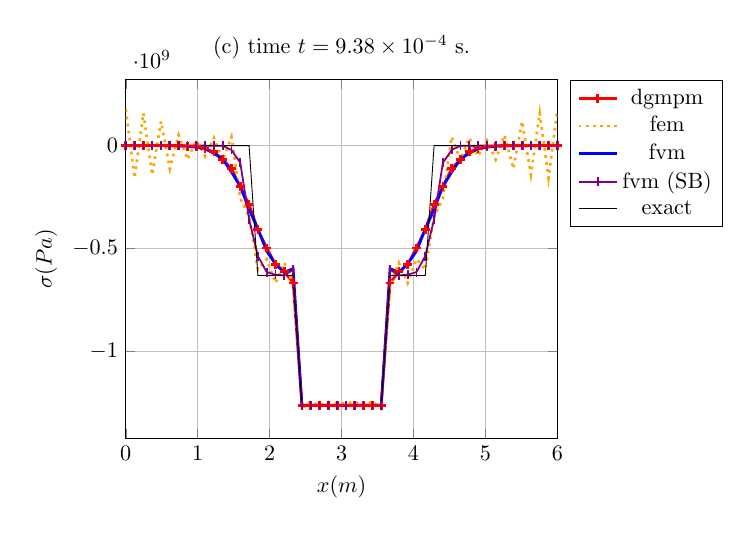
\begin{tikzpicture}[scale=0.8]
\begin{axis}[xlabel=$x (m)$,ylabel=$\sigma (Pa)$,ymajorgrids=true,xmajorgrids=true,legend pos=outer north east,title={(c) time $t = 9.38\times 10^{-4} $ s.},xmin=0.,xmax=6.]
\addplot[Red,very thick,mark=+,solid] coordinates {(0.0,-288.000337932026) (0.12244897959183673,-2340.8049612902105) (0.24489795918367346,-6717.6736351549625) (0.36734693877551017,-31436.18543893099) (0.4897959183673469,-82819.9714218378) (0.6122448979591837,-326370.9123286009) (0.7346938775510203,-787154.078435719) (0.8571428571428571,-2592039.5752673745) (0.9795918367346939,-5646941.091449857) (1.1020408163265305,-15363721.703146875) (1.2244897959183674,-29743749.6379236) (1.346938775510204,-65953645.19968581) (1.4693877551020407,-111309952.1584177) (1.5918367346938775,-198327314.77079153) (1.7142857142857142,-286130814.5665445) (1.836734693877551,-406728211.7590298) (1.9591836734693877,-496866659.9258773) (2.0816326530612246,-575814412.3291713) (2.204081632653061,-612581021.5556202) (2.326530612244898,-666589640.9783583) (2.4489795918367347,-1261004576.2605588) (2.571428571428571,-1261004576.2605588) (2.693877551020408,-1261004576.2605588) (2.816326530612245,-1261004576.2605593) (2.9387755102040813,-1261004576.2605593) (3.061224489795918,-1261004576.2605588) (3.183673469387755,-1261004576.2605584) (3.306122448979592,-1261004576.2605593) (3.4285714285714284,-1261004576.2605581) (3.5510204081632653,-1261004576.2605588) (3.673469387755102,-666589640.9783561) (3.7959183673469385,-612581021.5556188) (3.9183673469387754,-575814412.3291719) (4.040816326530612,-496866659.9258761) (4.163265306122449,-406728211.75903) (4.285714285714286,-286130814.5665426) (4.408163265306122,-198327314.77079123) (4.530612244897959,-111309952.15841806) (4.653061224489796,-65953645.19968575) (4.775510204081632,-29743749.637924016) (4.8979591836734695,-15363721.703146577) (5.020408163265306,-5646941.091449976) (5.142857142857142,-2592039.5752685666) (5.26530612244898,-787154.0784354806) (5.387755102040816,-326370.91232824326) (5.5102040816326525,-82819.97142159939) (5.63265306122449,-31436.185439646244) (5.755102040816326,-6717.673635229468) (5.877551020408163,-2340.804961979389) (6.0,-288.00033782143146) };
\addplot[Orange,very thick,mark=none,dotted] coordinates {(0.0011999999999999927,175010887.86141148) (0.12359999999999997,-157010320.72319484) (0.24599999999999994,157731015.99830914) (0.36839999999999995,-141347084.0250168) (0.4907999999999999,117914146.10742596) (0.6131999999999999,-112262666.61428112) (0.7355999999999999,51745557.76652613) (0.858,-67268258.78012908) (0.9803999999999998,25135893.71762538) (1.1027999999999998,-51161038.25586742) (1.2251999999999996,38244096.87732005) (1.3475999999999997,-71286114.06399637) (1.4699999999999998,42529781.300441384) (1.5923999999999996,-256057713.884533) (1.7147999999999997,-344993293.7306862) (1.8371999999999995,-602082756.2554108) (1.9595999999999996,-551416188.3408538) (2.0819999999999994,-667542863.5679615) (2.2043999999999997,-569236978.9147782) (2.3267999999999995,-673381420.6974866) (2.4491999999999994,-1276652083.3178082) (2.5715999999999997,-1242412632.5978575) (2.6939999999999995,-1262303877.9393654) (2.8163999999999993,-1245296647.9512377) (2.9387999999999996,-1251720925.4068818) (3.0611999999999995,-1251720925.406923) (3.1835999999999993,-1245296647.951198) (3.305999999999999,-1262303877.9393706) (3.4283999999999994,-1242412632.5978665) (3.5507999999999993,-1276652083.3177838) (3.673199999999999,-673381420.6975331) (3.7955999999999994,-569236978.9147345) (3.9179999999999993,-667542863.5679996) (4.040399999999999,-551416188.3408496) (4.1628,-602082756.2553713) (4.2852,-344993293.7307386) (4.4076,-256057713.88448328) (4.53,42529781.300438166) (4.6524,-71286114.06398582) (4.7748,38244096.877307296) (4.8972,-51161038.2558347) (5.0196,25135893.71758467) (5.142,-67268258.78007948) (5.2644,51745557.766474634) (5.3868,-112262666.6142239) (5.5092,117914146.10736191) (5.6316,-141347084.02495122) (5.754,157731015.9982485) (5.8764,-157010320.7231324) (5.9988,175010887.86135092) };
\addplot[Blue,very thick,mark=none,solid] coordinates {(0.0011999999999999927,-672.000788774134) (0.12359999999999997,-2317.190485430212) (0.24599999999999994,-11624.7450740413) (0.36839999999999995,-31435.028274873635) (0.4907999999999999,-131180.5918317446) (0.6131999999999999,-326370.86669091054) (0.7355999999999999,-1145540.9690250745) (0.858,-2592039.5738099255) (0.9803999999999998,-7576352.574992208) (1.1027999999999998,-15363721.703109615) (1.2251999999999996,-36933763.60530679) (1.3475999999999997,-65953645.19968625) (1.4699999999999998,-128588545.2855558) (1.5923999999999996,-198327314.77079248) (1.7147999999999997,-310077223.60174906) (1.8371999999999995,-406728211.759032) (1.9595999999999996,-512542911.78098124) (2.0819999999999994,-575814412.329173) (2.2043999999999997,-615644905.6578237) (2.3267999999999995,-597093014.0061195) (2.4491999999999994,-1261004576.2605588) (2.5715999999999997,-1261004576.2605586) (2.6939999999999995,-1261004576.2605588) (2.8163999999999993,-1261004576.2605584) (2.9387999999999996,-1261004576.2605588) (3.0611999999999995,-1261004576.2605586) (3.1835999999999993,-1261004576.2605586) (3.305999999999999,-1261004576.2605586) (3.4283999999999994,-1261004576.2605588) (3.5507999999999993,-1261004576.2605584) (3.673199999999999,-597093014.0061196) (3.7955999999999994,-615644905.6578233) (3.9179999999999993,-575814412.329173) (4.040399999999999,-512542911.78098106) (4.1628,-406728211.759032) (4.2852,-310077223.601749) (4.4076,-198327314.77079242) (4.53,-128588545.28555562) (4.6524,-65953645.199686386) (4.7748,-36933763.60530707) (4.8972,-15363721.703109678) (5.0196,-7576352.5749919815) (5.142,-2592039.5738102393) (5.2644,-1145540.9690254903) (5.3868,-326370.8666910869) (5.5092,-131180.5918318261) (5.6316,-31435.028275203294) (5.754,-11624.74507411075) (5.8764,-2317.1904855701214) (5.9988,-672.0007888251785) };
\addplot[Purple,thick,mark=|,solid] coordinates {(0.0011999999999999927,-2.2554342869669835e-07) (0.12359999999999997,-4.253451172600671e-07) (0.24599999999999994,-1.2920591556701192e-05) (0.36839999999999995,-5.986342632906781e-05) (0.4907999999999999,-0.0056401329400634255) (0.6131999999999999,-0.02444787812144389) (0.7355999999999999,-1.8760696294301331) (0.858,-7.9566149629172855) (0.9803999999999998,-503.4524595203254) (1.1027999999999998,-2086.1665527314763) (1.2251999999999996,-111480.01946610014) (1.3475999999999997,-452326.4024975486) (1.4699999999999998,-21130457.36149759) (1.5923999999999996,-83990511.6868726) (1.7147999999999997,-358373061.4587475) (1.8371999999999995,-536458450.92552686) (1.9595999999999996,-614366251.640357) (2.0819999999999994,-627343167.840607) (2.2043999999999997,-630228089.3811917) (2.3267999999999995,-602429197.2873981) (2.4491999999999994,-1261004576.2605584) (2.5715999999999997,-1261004576.2605586) (2.6939999999999995,-1261004576.2605581) (2.8163999999999993,-1261004576.2605586) (2.9387999999999996,-1261004576.2605584) (3.0611999999999995,-1261004576.2605586) (3.1835999999999993,-1261004576.2605584) (3.305999999999999,-1261004576.2605588) (3.4283999999999994,-1261004576.2605584) (3.5507999999999993,-1261004576.2605586) (3.673199999999999,-602429197.287398) (3.7955999999999994,-630228089.3811923) (3.9179999999999993,-627343167.8406069) (4.040399999999999,-614366251.6403568) (4.1628,-536458450.9255258) (4.2852,-358373061.45874953) (4.4076,-83990511.68687272) (4.53,-21130457.361496225) (4.6524,-452326.4024989642) (4.7748,-111480.01946637034) (4.8972,-2086.166552579263) (5.0196,-503.4524587330095) (5.142,-7.956613651988789) (5.2644,-1.8760695971344141) (5.3868,-0.024446596221118888) (5.5092,-0.005640085558921308) (5.6316,-6.008348006163438e-05) (5.754,-1.352714115819129e-05) (5.8764,-1.6124271861316672e-09) (5.9988,-1.7267558828412451e-07) };
\addplot[black,thin,mark=none,solid] coordinates {(0.0,-0.0) (0.12244897959183673,-0.0) (0.24489795918367346,-0.0) (0.36734693877551017,-0.0) (0.4897959183673469,-0.0) (0.6122448979591837,-0.0) (0.7346938775510203,-0.0) (0.8571428571428571,-0.0) (0.9795918367346939,-0.0) (1.1020408163265305,-0.0) (1.2244897959183674,-0.0) (1.346938775510204,-0.0) (1.4693877551020407,-0.0) (1.5918367346938775,-0.0) (1.7142857142857142,-0.0) (1.836734693877551,-630502288.1302795) (1.9591836734693877,-630502288.1302795) (2.0816326530612246,-630502288.1302795) (2.204081632653061,-630502288.1302795) (2.326530612244898,-630502288.1302795) (2.4489795918367347,-1261004576.260559) (2.571428571428571,-1261004576.260559) (2.693877551020408,-1261004576.260559) (2.816326530612245,-1261004576.260559) (2.9387755102040813,-1261004576.260559) (3.061224489795918,-1261004576.260559) (3.183673469387755,-1261004576.260559) (3.306122448979592,-1261004576.260559) (3.4285714285714284,-1261004576.260559) (3.5510204081632653,-1261004576.260559) (3.673469387755102,-630502288.1302795) (3.7959183673469385,-630502288.1302795) (3.9183673469387754,-630502288.1302795) (4.040816326530612,-630502288.1302795) (4.163265306122449,-630502288.1302795) (4.285714285714286,-0.0) (4.408163265306122,-0.0) (4.530612244897959,-0.0) (4.653061224489796,-0.0) (4.775510204081632,-0.0) (4.8979591836734695,-0.0) (5.020408163265306,-0.0) (5.142857142857142,-0.0) (5.26530612244898,-0.0) (5.387755102040816,-0.0) (5.5102040816326525,-0.0) (5.63265306122449,-0.0) (5.755102040816326,-0.0) (5.877551020408163,-0.0) (6.0,-0.0) };
\legend{dgmpm,fem,fvm,fvm (SB),exact}
\end{axis}
\end{tikzpicture}
%%% Local Variables:
%%% mode: latex
%%% TeX-master: "../../mainManuscript"
%%% End:
